\documentclass[12pt]{article}

\setlength\parindent{0pt}
\newcommand{\myt}[1]{\textbf{\underline{#1}}}

\usepackage{mathtools}
\usepackage{amssymb}
\usepackage{graphicx}

\title{\vspace{-15ex}Math 239 Lecture 18\vspace{-1ex}}
\date{June 17th, 2015}
\author{Graham Cooper}

\begin{document}
	\maketitle
	
	\section*{Special Graphs}
	\subsection*{Bipartite}
	
	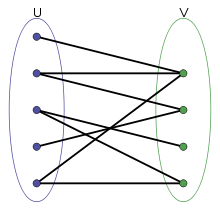
\includegraphics[scale=0.5]{bipartite.png}
	
	For m,n $\in$ N, the complete bipartite graph, $K_{m,n}$ with bipartition (A,B) where $|A|$ = m, $|B|$ = n and it contains all possible edges joining a vertex in A with a vertex in B\\
	
	How many edes are in $K_{m,n}$? mn, m chocies for a vertex in A, each paired with teh n ertices in B.\\
	
	\subsection*{N-cube}
	The n-cube is the graph where the vertices are all binary strings of length n, and two strings are adjacent if and only if they differe in exactly one bit.\\
	
	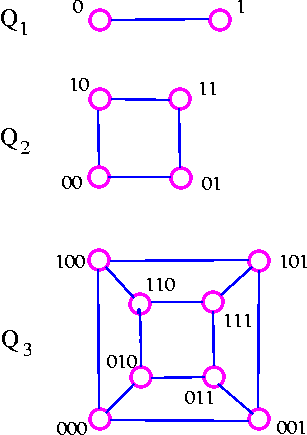
\includegraphics[scale=0.5]{n-cube.png}
	
	Properties of the n-cube:
	\begin{enumerate}
		\item $2^n$ vertices
		\item n-regular. For a string of length n, we can change one of the n-bits to get a neighbour $\implies$ degree n
		\item $\frac{n\cdot 2^n}{2} = n \cdot 2^{n-1}$ edges. Total degree is n $\cdot 2^n$ by handshaking lemma, the number of edges is half of it.
		\item It is bipartite. Consider the bipartition (A,B) where:\\
				A consists of strings with even number of 1's and \\
				B consists of strings with odd number of 1's\\
				Let s,t be strings where st is an edge. Suppose wlog $s \in A$. We get t be either chaning a 0 to a 1 (increases number of 1s by 1) or changing a 1 to a 0 (decrease numbre of 1's by 1). Since s has even number of 1s t must have an odd number of 1's. So $t \in B$. Therefoe the n-cube is bipartite.
	\end{enumerate}
	
	Recursive construction of the n-cube:
	\begin{enumerate}
		\item Take 2 copies of the (n-1)-cube
		\item Attach 0 in front of all strings in one copy, attach a 1 in front of all strings in the other copy
		\item Join corresponding vertices withedges.
	\end{enumerate}
	
	End of midterm material!!!!
	
	
	
\end{document}
